\documentclass[a4paper,10pt,twocolumn]{article}

\usepackage[utf8x]{inputenc}
\usepackage[french]{babel}
\usepackage{graphicx,times}
\usepackage[T1]{fontenc}
\usepackage{amsmath,amssymb}
\usepackage[font=footnotesize]{caption}
\usepackage{fancyhdr}
\usepackage[explicit]{titlesec}
\usepackage{hyperref}
\usepackage[square,comma,numbers]{natbib}
\usepackage{tabularx}
\usepackage{xcolor}

% bleu (légèrement turquoise)
\definecolor{darkblue1}{hsb}{.6,1,.5}

%for columns spanning multiple rows in tables
\usepackage{multirow}
%use the booktabs package to get (much!) better vertical spacing above and below "rules" (horizontal lines), resulting in a much more professional look of your tables.
%use the colortbl package to add color to tables.
\usepackage{booktabs,colortbl}

% fix problem with ":" in bibtex keys
% cf http://tex.stackexchange.com/questions/130344/using-citep-leads-to-missing-endcsname-inserted-error
\makeatletter
\let\ORG@NAT@sort@cites\NAT@sort@cites
\def\NAT@sort@cites#1{%
  \edef\@tempa{\detokenize{#1}}%
  \ORG@NAT@sort@cites\@tempa
}
\makeatother

% Petits extras:
\usepackage{textcomp} % Symbole Euro € \texteuro

\providecommand{\abs}[1]{\lvert#1\rvert}
\providecommand{\norm}[1]{\lVert#1\rVert}
\providecommand{\avg}[1]{\langle#1\rangle}

% Typographie:
\newcommand\tsp[1]{\textsuperscript{#1}}
\newcommand\sub[1]{\textsubscript{#1}}
\newcommand\kWc{kW\sub{c}{}} % point médian
\newcommand\tpc{\textperiodcentered} % point médian

% détails, en gris: (e.g. std in table)
\providecommand{\deta}[1]{\textcolor{gray}{#1}}



\newcolumntype{L}[1]{>{\raggedright\arraybackslash}p{#1}}
\newcolumntype{C}[1]{>{\centering\arraybackslash}p{#1}}
\newcolumntype{R}[1]{>{\raggedleft\arraybackslash}p{#1}}

%\renewcommand{\bibsection}{}
%\def\bibfont{\footnotesize}
\setlength{\bibsep}{0.3em}
%\setlength{\bibhang}{10em}

\hypersetup{colorlinks=true,
urlcolor=darkblue1,
linkcolor=darkblue1,
citecolor=black,
}

%\hypersetup{colorlinks=true, urlcolor=blue, urlbordercolor={0 0 1}, citecolor=black, citebordercolor={1 1 1}}

\addto\captionsfrench{\def\figurename{Fig.}}
\addto\captionsfrench{\def\tablename{Tableau}}

\captionsetup[figure]{labelsep=period, justification=raggedright, singlelinecheck=false}
\captionsetup[table]{labelsep=period, justification=centering, singlelinecheck=false}

\parindent 10pt

\setlength{\voffset}{-1.3in}
\setlength{\topmargin}{1.25cm}
\setlength{\headheight}{1.125cm}
\setlength{\headsep}{0cm}

\setlength{\hoffset}{-1in}
\setlength{\oddsidemargin}{1.3cm}
\setlength{\evensidemargin}{1.3cm}

\setlength{\textheight}{25cm}%23.5
\setlength{\textwidth}{18.5cm}

\setlength{\headsep}{0.67cm}
\setlength{\columnwidth}{8.75cm}
\setlength{\columnsep}{0.63cm}

\setlength{\abovecaptionskip}{0em}
\setlength{\belowcaptionskip}{0em}

\titleformat{\section}
  {\normalfont}{\thesection.}{0.5em}{\MakeUppercase{#1}}
\titleformat{\subsection}
  {\normalfont\itshape}{\thesubsection.}{1.5em}{#1}
\titleformat{\subsubsection}
  {\normalfont\itshape}{\thesubsubsection.}{1.5em}{#1}
	
\titlespacing\section{0pt}{1em}{0.5em}
\titlespacing\subsection{0pt}{1em}{0.5em}
\titlespacing\subsubsection{0pt}{1em}{0.5em}

\fancyhf{}
\fancyhead[R]{\fontsize{8pt}{8pt}\selectfont \textbf{S}YMPOSIUM DE \textbf{G}ENIE \textbf{E}LECTRIQUE (SGE 2018), 3-5 JUILLET 2018, NANCY, FRANCE}
\renewcommand{\headrulewidth}{0pt}


\pagestyle{empty}


\title{
\fontsize{24pt}{24pt}\selectfont
Gestion d'énergie avec entrées incertaines : \\
quel algorithme choisir ?\\
Benchmark open source sur une maison solaire
}

\author{
\fontsize{11pt}{11pt}\selectfont
Pierre HAESSIG\tsp{*}, Jesse James PRINCE AGBODJAN\tsp{*}, Romain BOURDAIS\tsp{*}, Hervé GUÉGUEN\tsp{*}\\
\fontsize{10pt}{10pt}\selectfont
\tsp{*}IETR, CentraleSupélec
}

\date{}


\begin{document}

\maketitle
\thispagestyle{fancy}


\fontsize{9pt}{9pt}\selectfont
\textbf{RÉSUME --
Le pilotage optimal des systèmes énergétiques nécessite des stratégies
de gestion basées sur des algorithmes d'optimisation.
La palette d'outils est large, or chaque outil fait appel à des théories variées
(optimisation convexe, dynamique, stochastique...)
qui nécessitent chacune un temps d'appropriation allant de quelques jours à plusieurs mois.
%
Il est donc difficile, pour le ou la praticien\tpc{}ne novice en gestion d'énergie
de saisir les principales caractéristiques de chaque approche
pour pouvoir les comparer objectivement et finalement trouver
la ou les méthodes les plus adaptées à un problème donné.
%
Pour faciliter une comparaison objective et transparente,
nous proposons un problème de gestion d'énergie emblématique et simple : une maison solaire
avec production photovoltaïque et stockage.
Après avoir justifié le dimensionnement du système,
nous illustrons le benchmark par une première comparaison de quelques méthodes de gestion d'énergie
(règle heuristique, MPC et optimisation anticipative).
Nous soulignons en particulier l'effet de l'incertitude de la production solaire
sur la performance.
Ce benchmark, avec les méthodes de gestion décrites,
est open source, accessible en ligne et multi-langage (Python, Julia et Matlab).
% Extrait de l'ancien résumé, avec des idées à reprendre?
% comparer différentes méthodes en soulignant en particulier les investissements
% en temps à prévoir :
% temps pour la compréhension du cadre théorique,
% temps pour la modélisation du problème dans ce cadre,
% temps pour l'implémentation numérique et la validation des résultats.
}\\

\textbf{\textit{Gestion d'énergie, Optimisation dynamique,
Commande prédictive, Dimensionnement, Autoconsommation photovoltaïque.}}

\fontsize{10pt}{10pt}\selectfont


\section{Introduction}

De très nombreux travaux de recherche portent sur le pilotage des systèmes énergétiques
pour optimiser leur fonctionnement.
Les méthodes de gestion d'énergie sont nombreuses et variées (cf. partie \ref{s:opt_meth}).
Ainsi, la personne qui aborde un problème de gestion d'énergie
est confrontée à un choix qui est souvent difficile à \emph{objectiver}.
En effet, les difficultés associées à chaque méthode sont de nature diverse:
difficultés de compréhension du cadre théorique, difficultés d'implémentation
numérique ou de temps de calcul, et parfois existence de
``dépendances cachées''\footnote{
  exemple de dépendance : la méthode ``commande prédictive'' (MPC)
  nécessite une prévision des entrées incertaines,
  à générer si l'on n'en dispose pas déjà, cf. partie \ref{ss:mpc}.}.
Malheureusement, les méthodes a priori les plus performantes du point de vue de l'optimalité
cumulent la plupart de ces difficultés.
Dès lors, la personne face au choix pourrait avoir peur d'investir beaucoup de son temps
dans une méthode ``complexe'' si elle n'a pas une certaine assurance d'obtenir une meilleure
performance qu'avec une méthode ``simple''.

Pour sortir de ce dilemme, nous souhaitons faciliter la \emph{comparaison objective},
sans préjugés, des méthodes de gestion d'énergie.
Nous proposons donc un \emph{banc de test de gestion d'énergie open source}.
Il permet, sur un exemple simple, mais pertinent, d'avoir un aperçu de différentes méthodes
de pilotage\footnote{``pilotage'', ``gestion'', ``commande'', ``optimisation''...
le vocabulaire change selon les disciplines ou le contexte.
Nous utilisons ici ces termes de façon interchangeable.}.
Ce benchmark doit permettre de les comparer
à la fois du point de vue de la performance (optimalité du résultat),
mais aussi de comparer leur mise en oeuvre, en particulier l'implémentation
dans différents langages de programmation (complexité du code source, dépendances logicielles).

Il existe des travaux comparant des méthodes de gestion d'énergie, sur des exemples réels complexes
(barrages hydroélectriques \cite{Zambelli:2011:SBA}, véhicules hybrides \cite{Jiang:2017:ToVT}).
Notre proposition est complémentaire, car elle porte au moins autant sur la comparaison \emph{fonctionnelle}
des méthodes (e.g. analyse des objets nécessaires pour leur mise en oeuvre) que
sur la comparaison quantitative des résultats d'optimisation.
Par ailleurs, notre proposition est librement accessible à tous (code et données open source).

\section{Banc de test: maison solaire}

\subsection{Modèle de la maison solaire}
\label{ss:model}

\begin{figure}[!ht]
        \begin{center}
                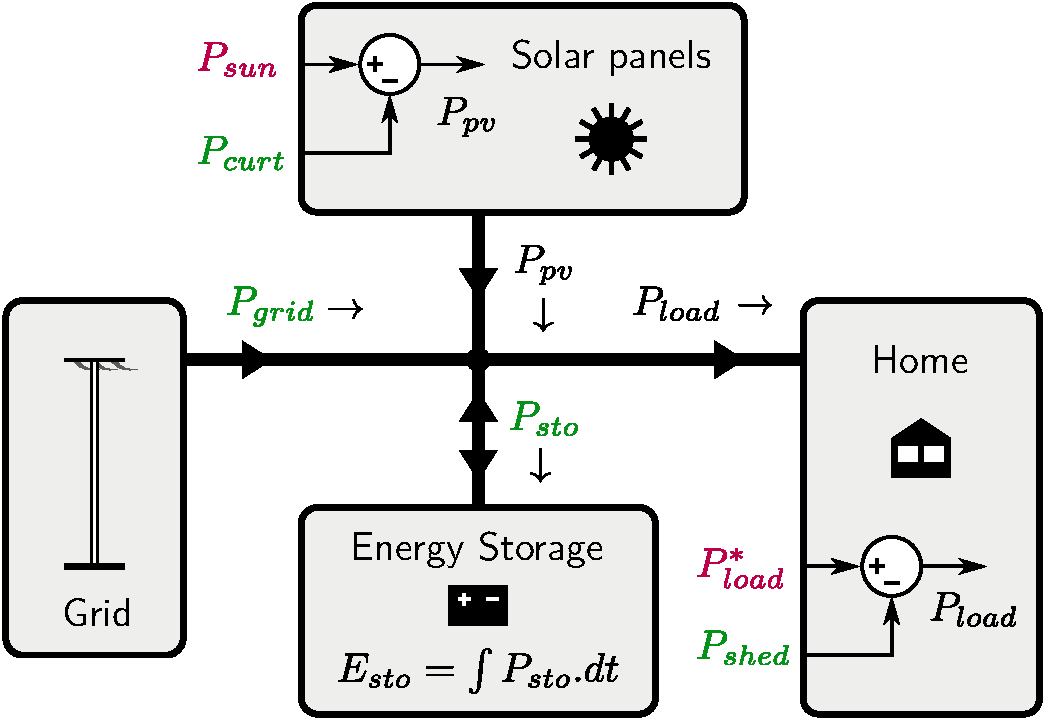
\includegraphics[width=0.9\columnwidth]{figures/solar_home.pdf}
        \end{center}

        \caption{Modèle en flux d'énergie de la maison solaire.
        Variables de décision en vert, données externes en rouge (potentiel solaire et consommation souhaitée), variables internes en noir.
        La consommation du foyer $P_{load}^*$, imposée, est couverte par 3 sources:
        le réseau électrique, des panneaux solaires (délestables)
        et un système de stockage.
        En dernier recours, la consommation de la maison peut être délestée.
        }
        \label{fig:solhome}
\end{figure}

Pour illustrer les différentes méthodes de gestion d'énergie à comparer,
nous avons choisi un système ``banc de test'' qui soit à la fois simple et concret.
Nous considérons une maison solaire modélisée par
des flux d'énergie (figure \ref{fig:solhome}).
Il s'agit d'un modèle simple de système photovoltaïque avec stockage
pour l'autoconsommation d'un consommateur résidentiel connecté au réseau.
Le modèle s'exprime à temps discret (instant $k$ entier),
avec un pas de temps $\Delta_t$. On note $n$ la durée du test
en nombres de pas.

L'objectif de pilotage est la minimisation de la facture d'électricité,
c'est-à-dire le coût de l'énergie consommée du réseau:

\begin{equation} \label{eq:C_grid}
  C_{grid} = \sum_{k=1}^{n} c_{grid}(k)P_{grid}(k)
\end{equation}

où $c_{grid}$ est le prix de l'énergie (\texteuro/kWh), potentiellement variable,
mais supposé connu à l'avance.

\subsubsection{Données du problème}
\label{sss:fixed_var}

La stratégie de gestion qui minimise le coût \eqref{eq:C_grid}
dépend pour commencer des variations du prix de l'électricité $c_{grid}$ (€/kWh).
Nous avons choisi un signal connu à l'avance, fonction de l'heure du jour,
avec deux niveaux de prix:
\begin{itemize}
 \item $c_{night}$ : heures creuses la nuit, de 0h00 à 6h00
 \item $c_{day}$ : heures pleines la journée à partir de 6h00
\end{itemize}

Formellement, l'heure du jour $hod$ (``hour of the day'') est définie par:
%
\begin{equation} \label{eq:hod}
  hod = t \; \% \; 24 \in [0, 24[
\end{equation} 
où $t$ est le temps exprimé en heures, avec $t=0$ calé à minuit.
Le prix est alors défini par morceaux, fonction de $hod$:
\begin{equation}
  c_{grid}(hod) = \begin{cases}
    c_{night} = 0.10 \text{ €/kWh} & \text{ pour } 0 \leq hod < 6\text{ h}\\
    c_{day} \;\;\,  = 0.20 \text{ €/kWh} & \text{ pour } 6 \leq hod < 24\text{ h}
  \end{cases}
\end{equation}

Pour avoir un effet heures pleines / heures creuses vraiment incitatif,
nous avons choisi des prix nettement différents.

Le signal prix pourrait bien sûr être complexifié avec plus de niveaux de prix
(par exemple avec des ``heures de pointe''), et une dépendance au jour de la semaine
(par exemple un tarif semaine / weekend).
Il serait aussi possible de faire payer l'énergie plus cher lorsque la puissance
dépasse la puissance réseau souscrite\footnote{
  principe de la pénalité de dépassement de l'ancien ``tarif vert'' d'EDF}
(tarif vertueux pour réduire la puissance souscrite).

En plus du signal prix, les données du problème (en rouge sur la figure \ref{fig:solhome}) sont:

\begin{itemize}
 \item $P_{sun}$ : productible solaire, c'est-à-dire la production des panneaux en régime
MPPT\footnote{Maximum power point tracking}
 \item $P_{load}^*$ : consommation souhaitée par la maison
\end{itemize}

À l'inverse du prix, ces deux signaux ne sont pas connus à l'avance :
ce sont des \emph{entrées incertaines}.
Cela signifie qu'à un instant de la simulation, le choix des variables
de décisions ne peut dépendre que des valeurs passées de ces variables
(contrainte de non-anticipativité).
Le jeu de donnée source est décrit partie \ref{ss:sol_data}.

Le problème s'appuie aussi sur trois paramètres fixes:
\begin{itemize}
 \item capacité de la batterie $E_{rated}$ (kWh)
 \item puissance nominale des panneaux $P_{PVp}$ (\kWc)
 \item puissance réseau souscrite $P_{grid}^{max}$ (kW)
\end{itemize}

La valeur des paramètres est donnée dans le tableau \ref{tab:dim_stats}.
L'origine de ces valeurs, c'est-à-dire le dimensionnement de la maison solaire,
est détaillée partie \ref{ss:dimens}.

\subsubsection{Variables de décision}
\label{sss:opti_var}

Les degrés de liberté du problème (en vert sur la figure) sont au nombre de quatre.
La puissance soutirée du réseau, $P_{grid}$,
est limitée par la puissance souscrite
et l'injection est interdite\footnote{
équivalent, du point de vue de l'optimisation, à autoriser l'injection, mais sans la rémunérer}:
%
\begin{equation}
  0 \leq P_{grid} \leq P_{grid}^{max}
\end{equation}
%
Le système de gestion d'énergie peut tirer profit de l'énergie, marginalement
gratuite, produite par les panneaux solaires $P_{pv}$.
Cette puissance est librement réglable entre 0 et $P_{sun}$ grâce à la variable
d'écrêtage $P_{curt}$ :
%
\begin{equation}
  P_{pv} = P_{sun} - P_{curt}, \text{ avec } 0 \leq P_{curt} \leq P_{sun}
\end{equation}

Le système de gestion peut enfin exploiter le degré de liberté offert par
le système de stockage qui permet de décaler, au moins partiellement,
la production solaire et la consommation.
Le stockage, dont on néglige les pertes, est modélisé par l'énergie qu'il contient:
%
\begin{equation}
  E_{sto}(k+1) = E_{sto}(k) + P_{sto}(k)\Delta_t
\end{equation}
%
et cette énergie est limitée par la capacité de stockage :
%
\begin{equation}
  0 \leq E_{sto} \leq E_{rated}
\end{equation}

Tous les flux sont liés par la conservation de l'énergie:

\begin{equation} \label{eq:cons}
  P_{grid} + \underbrace{P_{sun} - P_{curt}}_{P_{pv}} = P_{load} + P_{sto}
\end{equation}

La consommation $P_{load}$ a vocation à suivre la consommation souhaitée $P_{load}^*$
(pas de charges ``intelligentes'' déplaçables), et dans tout cet article, ces deux
variables seront égales et donc assimilés.
Nous définissons cependant $P_{shed}$ comme un délestage de dernier
recours pour les situations critiques\footnote{faible puissance souscrite, lorsque
la batterie est vide et qu'il n'y a que peu de soleil} et qui permet
de ramener $P_{load}$ à zéro si nécessaire:
%
\begin{equation}
  P_{load} = P_{load}^* - P_{shed}, \text{ avec } 0 \leq P_{shed} \leq P_{load}^*
\end{equation}

Si ce quatrième degré de liberté doit être utilisé,
alors il faut l'ajouter comme pénalité dans la fonction coût \eqref{eq:C_grid}.

\subsubsection{Variables auxiliaires}
\label{sss:auxi_var}

Deux grandeurs auxiliaires sont utiles pour l'analyse de la gestion d'énergie.
Tout d'abord, la charge nette $P_{nl}$ (``net load'') qui est la différence
entre la charge souhaitée et le productible solaire:
%
\begin{equation}
  P_{nl} \triangleq P_{load}^* - P_{sun}
\end{equation} 
%
Nous verrons qu'elle est fondamentale pour définir une gestion d'énergie heuristique
(partie \ref{ss:heuris}).

Ensuite, nous définissons $P_{gc}$ comme la différence entre deux variables
de décision, la puissance réseau et l'écrêtage:
%
\begin{equation}
  P_{gc} \triangleq P_{grid} - P_{curt}
\end{equation} 

Cette variable condense la décision de la loi de gestion.
Nous tirons parti du fait que $P_{grid}$ et $P_{curt}$ sont exclusives,
c'est-à-dire que l'une est $>0$ lorsque l'autre est nulle.

Avec ces variables, l'équation de conservation de la puissance \eqref{eq:cons}
se simplifie en:
%
\begin{equation} \label{eq:cons2}
  P_{gc} - P_{sto} = P_{nl}
\end{equation}
%
%et cette écriture présente l'intérêt de regrouper les données d'entrée
%d'une part et les variables de décision de l'autre. côte


\subsection{Dimensionnement de la maison solaire}
\label{ss:dimens}

La performance d'un système photovoltaïque-stockage dépend certes de la loi de gestion,
mais aussi très fortement de son dimensionnement
(capacité de stockage $E_{rated}$,
puissance des panneaux $P_{PVp}$ et 
puissance souscrite $P_{grid}^{max}$).

La question de l'optimisation du dimensionnement, bien qu'intéressante,
n'est pas l'objet de notre banc de test, mais il est tout de même nécessaire
de trouver un dimensionnement ``raisonnable''.
%
Avant d'expliquer notre méthode de dimensionnement, voici une analyse
succincte de son résultat (tableau \ref{tab:dim_stats}) :

\begin{itemize}
 \item $P_{PVp}$ : Avec 4\,kW\sub{c} de panneaux, la production solaire couvre 91\%
de la consommation sur la période de test (avec bien sûr une forte variabilité journalière).
 \item $E_{rated}$ : La batterie de 8\,kWh correspond à environ la moitié de la consommation
 ou de la production solaire journalière.
 \item $P_{grid}^{max}$ : Les 3 kW de puissance réseau souscrite sont plus grands
 que la charge maximale journalière habituelle,
 car nous avons choisi de ne pas nous intéresser à la gestion d'une connexion réseau faible
 dans cette première version du test.
\end{itemize}

Notons que le dimensionnement dépend bien sûr des données
de consommation et de production solaire (cf. détail partie \ref{ss:sol_data}).

\begin{table}[!h]
%% increase table row spacing, adjust to taste
\renewcommand{\arraystretch}{1.2}

\caption{Paramètres de dimensionnement de la maison solaire
et moyennes statistiques des données d'entrée sur la période de test
(30 jours).
En gris, écarts-types sur l'estimation de ces moyennes,
calculés par bootstrap.}
\label{tab:dim_stats}

\noindent
\centering
  \begin{center}
    \begin{tabular}{l l l l}
      \toprule
      \multicolumn{2}{c}{Paramètres} & \multicolumn{2}{c}{Statistiques des données} \\
      \midrule
      $E_{rated}$       & 8 kWh  & $\avg{P_{load}^*}$ &    17,02 \deta{± 0.33} kWh/j\\
      $P_{PVp}$         & 4 \kWc  & $\avg{P_{sun}}$    &    15,60 \deta{± 0.96} kWh/j\\
      $P_{grid}^{max}$  & 3 kW   & $\avg{P_{nl}}$     & \;\,1,42 \deta{± 0.94} kWh/j\\
      \bottomrule
    \end{tabular}
  \end{center}
\end{table}

\subsubsection{Méthode de dimensionnement}

Pour arriver au dimensionnement (4\,\kWc, 8\,kWh), nous avons conduit une étude
de sensibilité sur les paramètres $P_{PVp}$ et $E_{rated}$, respectivement
entre 0 et 6\,\kWc (par pas de 0,167) et entre 0 et 20\,kWh (pas de 0,5).
Pour chaque paire de valeurs, nous avons simulé la maison solaire
en utilisant la loi de gestion ``règle heuristique simple'' (cf. section \ref{ss:heuris})
qui est très rapide à simuler (40 ms pour les 30 jours) et est optimale
du point de vue de la consommation d'énergie (mais pas de la facture).


\begin{figure}[!ht]
  \begin{center}
	  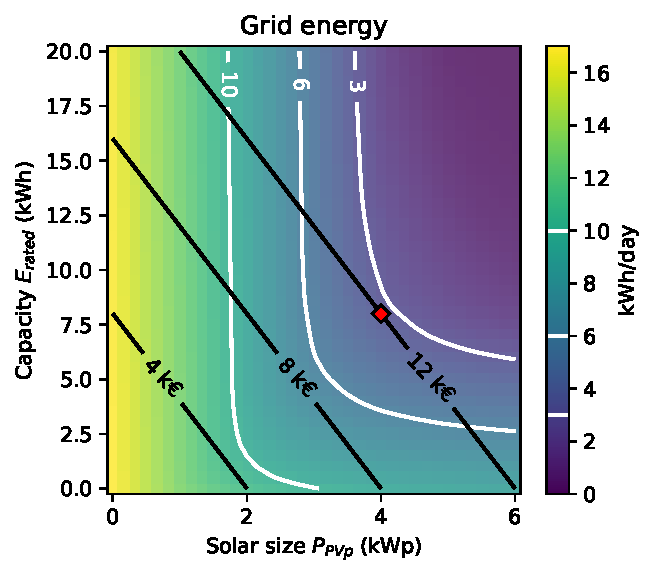
\includegraphics[width=0.8\columnwidth]{figures/Sizing_E_grid_invest_heatmap.pdf}
  \end{center}

  \caption{Effet du dimensionnement de la maison solaire sur sa consommation d'énergie réseau.
  Superposition des lignes d'iso-investissement.
  }
  \label{fig:P_grid_map}
\end{figure}

La figure \ref{fig:P_grid_map} donne la puissance moyenne consommée sur le réseau ($\avg{P_{grid}}$)
pour chaque dimensionnement. Celle-ci est égale à 17\,kWh/j sans PV ni batterie
et baisse à mesure que $P_{PVp}$ et $E_{rated}$ augmentent\footnote{
  Dans le détail,
  lorsque $E_{rated}=0$ la consommation baisse rapidement avec $P_{PVp}$
  tant qu'on ne dépasse pas 1 à 2\,\kWc. Pour intégrer davantage de PV,
  il faut ajouter une batterie.
  Inversement, pour $P_{PVp}=0$, la batterie seule ne permet pas de baisser la consommation.
  Elle pourrait néanmoins faire baisser la facture (en déplaçant la consommation)
  si une gestion optimale était employée.}.
Les isolignes de consommation (blanches) ont une forme coudée
et nous allons montrer pourquoi c'est \emph{au niveau d'un coude que le dimensionnement est optimal}.

Nous définissons un dimensionnement optimal comme celui qui minimise le coût global sur cycle de vie,
à savoir la somme du coût d'investissement $C_{inv}$
et du coût de fonctionnement opérationnel $C_{op}$:
%
\begin{equation} \label{eq:C_tot}
  C_{tot} = C_{inv} + C_{op}
\end{equation}


Le coût d'investissement est modélisé comme proportionnel à la puissance
des panneaux et la capacité de la batterie:
%
\begin{equation} \label{eq:C_inv}
  C_{inv} = c_P P_{PVp} + c_E E_{rated}
\end{equation} 
et nous avons choisi $c_E$ = 0.5 €/kWh (source : un Tesla Powerwall de 13,5 kWh s'affiche à 7 k€)
et $c_P$ = 2 €/\kWc{} (optimiste pour une petite installation de 4\,\kWc,
mais raisonnable pour une installation ``9 à 36 \kWc, ISB''\footnote{\url{http://www.photovoltaique.info/Couts-d-investissement.html}}).
Les isolignes d'investissement (noires) sont donc des droites inclinées
et le dimensionnement choisi coûte 12\,k€.

Le coût opérationnel $C_{op}$ est choisi égal à la facture d'électricité
sur le cycle de vie de l'installation (et donc proportionnel à la fonction-coût
du banc de test \eqref{eq:C_grid}).

\begin{equation} \label{eq:C_op}
  C_{op} = T_{life} \times \avg{c_{grid}.P_{grid} }
\end{equation} 

La durée de vie $T_{life}$ est égale à 20 ans (exprimée en heures).
Vu que nous avons choisi une loi de gestion heuristique qui ne gère pas les heures pleines et creuses,
nous avons choisi, pour le dimensionnement uniquement, un prix de l'électricité $c_{grid}$ fixe.
Par conséquent, le coût opérationnel \eqref{eq:C_op} est simplement proportionnel à
la consommation réseau moyenne ($\avg{P_{grid}}$).
On comprend alors pourquoi, à coût d'investissement donné (c.-à-d. sur une ligne noire figure \ref{fig:P_grid_map})
on a intérêt choisir le point qui tangente une courbe iso-consommation (blanche),
car il minimise le coût opérationnel. Cette tangence est obtenue dans un coude, comme annoncé plus haut.

Pour choisir le dimensionnement optimal, il existe deux méthodes :

\begin{itemize}
 \item soit choisir a priori un investissement initial et en déduire le dimensionnement
 dans le coude correspondant,
 \item soit choisir le dimensionnement qui minimise le coût global sur cycle de vie.
\end{itemize}

\begin{figure}[!ht]
  \begin{center}
	  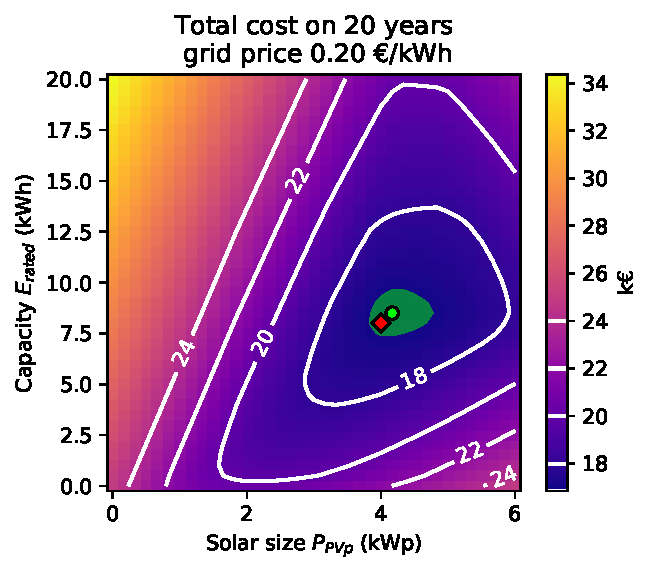
\includegraphics[width=0.8\columnwidth]{figures/Total_cost_map_grid020.pdf}
  \end{center}

  \caption{Effet du dimensionnement de la maison solaire sur son coût total sur cycle de vie
  (investissement + fonctionnement sur 20 ans).
  }
  \label{fig:cost_tot}
\end{figure}

Avec la 1\tsp{re} méthode, le résultat dépend du niveau d'investissement choisi.
Notre dimensionnement est l'optimum pour un investissement de 12\,k€.
Le dimensionnement le moins cher se situe autour du point
(1\,\kWc, 0\,kWh). Pour un investissement croissant,
le dimensionnement optimal se déplace approximativement le long
d'une demi-droite passant par (4\,\kWc, 8\,kWh), soit environ
2,7\,kWh/\kWc.
Au-delà du point (5\,\kWc, 11\,kWh), le réduction de consommation réseau devient très faible.

La 2\tsp{e} méthode est illustrée sur la figure \ref{fig:cost_tot},
pour un prix de l'électricité $c_{grid}$ = 0,20\,€/kWh.
Le dimensionnement que nous proposons (diamant rouge : 4\,kW\sub{c}, 8\,kWh)
est très proche de l'optimum (disque vert).
Il appartient en fait à la région quasi optimale (surlignée en vert)
où le coût total est inférieur à +1\% du minimum.
Le coût total d'environ 17\,k€ se répartit en 12\,k€ d'investissement
et 5\,k€ de fonctionnement (facture d'électricité sur 20 ans).

Ce résultat dépend fortement du choix de $c_{grid}$
(et de la durée d'amortissement $T_{life}$)
et nous avons donc répété l'analyse pour un prix entre 0,10 et 0,30\,€/kWh\footnote{%
  tracé animé de la figure \ref{fig:cost_tot} disponible sur le site du benchmarck}.
Il apparaît que notre dimensionnement est dans la zone quasi optimale pour un prix
compris entre 0,16 et 0,21\,€/kWh.


\subsection{Données de la maison solaire}
\label{ss:sol_data}

Notre banc de test est alimenté par le jeu de données \emph{réelles et ouvert}
``\href{https://www.ausgrid.com.au/Common/About-us/Corporate-information/Data-to-share/Solar-home-electricity-data.aspx}{Solar home electricity data}''
de l'opérateur Ausgrid (réseau de Sydney et sa région, Australie).
Il contient 3 années de consommation et production, au pas demi-horaire ($\Delta_t$ = 0,5\,h),
de 300 clients résidentiels disposants de panneaux PV.

Pour le banc de test, nous avons sélectionné le client sans charge pilotable\footnote{
  Client numéroté ``12''. La description détaillée de ce choix est fournie dans le fichier \href{https://github.com/pierre-haessig/solarhome-control-bench/blob/master/data/README.md}{data/README.md} du dépôt, avec plusieurs graphiques supplémentaires.
}
et nous avons choisi 30 jours consécutifs de test, du 29/11/2011 au 28/12/2011.
Les premiers jours de test sont représentés figure \ref{fig:testdata}.

La donnée de consommation est utilisée directement, mais
la donnée de productible solaire $P_{sun}$ nécessite une mise à l'échelle:
\begin{equation}
  P_{sun} = P_{PVp} \times P_{sun}^{1k} = P_{PVp}/1,04 \times GP 
\end{equation}
%
où $P_{sun}^{1k}$ correspond à la production potentielle d'un panneau de 1\,\kWc.
Elle est égale à $GP/1,04$ où $GP$ est la mesure de la production
dans le jeu de donnée original, et 1,04\,\kWc{} la taille de l'installation photovoltaïque
réelle du client choisi.

\begin{figure}[!ht]
        \begin{center}
                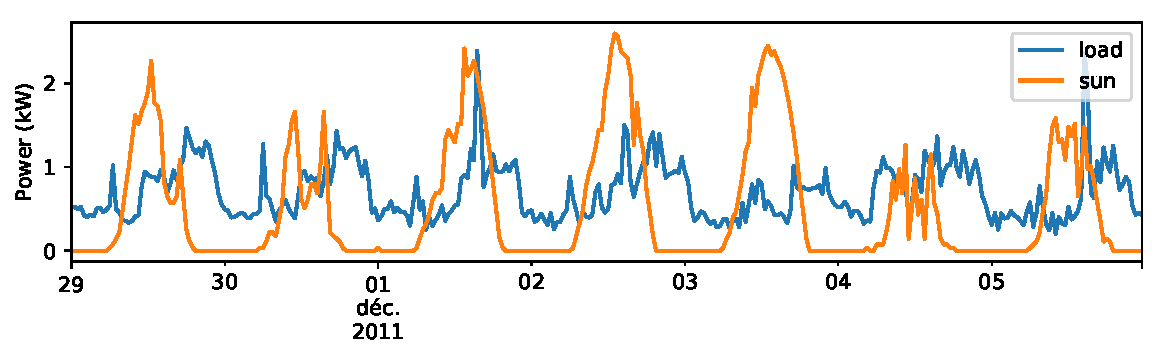
\includegraphics[width=1\columnwidth]{figures/data_week_2011-11-29.pdf}
        \end{center}

        \caption{Consommation et productible solaire durant les 7 premiers jours de test
        }
        \label{fig:testdata}
\end{figure}

Les données des 30 jours précédents sont également disponibles pour une phase d'apprentissage,
par exemple pour régler la prévision d'une commande prédictive.
L'enjeu est de bien respecter la stricte séparation entre ``training set''
et ``test set'', bien connue en machine learning, et qui permet d'éviter les effets de surapprentissage
(``overfitting'').

Le tableau \ref{tab:dim_stats} donne les moyennes statistiques du productible solaire $P_{sun}$
et de la consommation souhaitée $P_{load}^*$.
Nous avons choisi d'exprimer ces moyennes en kWh/jour pour que les valeurs soient indépendantes
des la durée du test (30\,j). De plus, cela permet de mettre en regard la capacité de la batterie
(8 kWh = 1/2 journée de consommation moyenne).

% TODO: speak about bootstrap

\subsection{Accès au banc de test open source}

La description de ce modèle ainsi que les données temporelles nécessaires sont
disponibles en open source dans le dépôt GitHub \href{https://github.com/pierre-haessig/solarhome-control-bench}{pierre-haessig/solarhome-control-bench}.
Ce dépôt contient également les implémentations des méthodes de gestion d'énergie présentées dans cet article.

Il a vocation à contenir des exemples dans les langages de programmation
parmi les plus utilisés pour ce type de problème:
Matlab, Python et Julia.

\section{Méthodes de gestion d'énergie}
\label{s:opt_meth}

Le but du banc de test ``maison solaire'' que nous proposons est de comparer
plusieurs lois de gestion de l'énergie pour minimiser la facture d'électricité \eqref{eq:C_grid}.
Nous présentons ici les premières stratégies que nous avons implémentées.
Le tracé temporel des 5 premiers jours du test est donné
figure \ref{fig:temporel}, pour trois méthodes différentes
que nous allons détailler.

\subsection{Contrôle par règle heuristique simple}
\label{ss:heuris}

La famille de méthode gestion par des règles simples (``rule-based control'')
est la plus simple à implémenter et la plus rapide à simuler.
La limite de cette approche, c'est qu'elle repose totalement
sur ``l'inspiration'' du concepteur, c'est-à-dire sa capacité à trouver
des heuristiques pertinentes.

Pour le cas de la maison solaire, si l'on s'en tient à minimiser
la consommation d'énergie (moyenne de $P_{grid}$),
par opposition à la facture (moyenne de $c_{grid}.P_{grid}$),
une stratégie très efficace consiste charger la batterie
avec le surplus solaire net (si production > consommation)
ou bien la décharger pour fournir la consommation nette (si consommation > production).
Formellement, ces deux actions s'écrivent en une équation :
%
\begin{equation} \label{eq:heuris_sto}
  P_{sto} = -P_{nl} = P_{sun} - P_{load}^*, \text{ ``tant que possible''}
\end{equation}
%
où ``tant que possible'' signifie que tant que la batterie n'est pas pleine ou vide,
selon le signe de $P_{nl}$
(variable auxiliaire définie partie \ref{sss:auxi_var}).
%
Si l'équation \eqref{eq:heuris_sto} est applicable, alors on déduit
de la conservation de la puissance \eqref{eq:cons2} que $P_{gc} = 0$,
c'est-à-dire $P_{grid} = 0$ (on ne consomme rien) et
$P_{curt} = 0$ (on ne gâche pas de productible solaire).
C'est bien une heuristique prometteuse, car cette décision est gratuite
sur l'instant.

Inversement, si \eqref{eq:heuris_sto} est inapplicable,
c'est que la batterie est saturée donc $P_{sto} = 0$
et la variable $P_{gc}$ sert de recours,
toujours pour assurer la conservation de la puissance \eqref{eq:cons2}:
%
\begin{equation}
  P_{gc} = P_{grid} - P_{curt} = P_{nl} = P_{load}^* - P_{sun}
\end{equation}

Comme $P_{grid}$ et $P_{curt}$ sont des variables de décision exclusives, deux sous-cas se présentent:
\begin{itemize}
 \item si $P_{nl}>0$ (c.-à-d. consommation > productible et batterie vide),
 le réseau prend le relais: $P_{grid} = P_{nl}$
 \item si $P_{nl}<0$ (c.-à-d. productible > consommation et batterie pleine),
 il faut écrêter la production: $P_{curt} = - P_{nl}$
 (ou autrement dit, $P_{pv}$ est ajustée égal à $P_{load}^*$)
\end{itemize}

Ce comportement est visible sur en haut de la figure \ref{fig:temporel},
où l'on observe que pendant une grande partie du temps,
la batterie suit la charge nette. Ainsi, elle se charge en cas d'excédent solaire,
elle se décharge si la consommation dépasse la production
et le recours $P_{gc}$ est constant égal à zéro.
Si la batterie est vide, et tant que la consommation domine,
le réseau prend le relais ($P_{gc}>0$, souligné en rouge)
Inversement si la batterie est pleine, et tant que la production solaire domine,
l'écrêtage intervient ($P_{gc}<0$, souligné en jaune).

L'analyse quantitative des résultats (tableau \ref{tab:perf_stats}, ligne ``heuristique'')
montre que la consommation d'énergie ($\avg{P_{grid}}$ = 3,38\,kWh/j) est minimale, car égale à celle de 
l'optimisation anticipative qui minimise la consommation, ligne ``optim. éner.''
(cf. partie \ref{ss:anticip}).
Par contre, la facture n'est pas optimale, car cette méthode ne tient pas compte
des heures creuses. D'ailleurs, on observe figure \ref{fig:temporel}
que l'appel au réseau ($P_{gc}>0$) ne se fait pas préférentiellement pendant
les périodes bleues clair.

La limite de cette méthode de gestion d'énergie est donc le pendant négatif
de sa simplicité : il est difficile d'intégrer des complexités du problème
tel que des tarifs flexibles.

% \subsection{Programmation dynamique}
% La programmation dynamique\cite{Bertsekas:2005:DPOC_vol1} est un
% excellent cadre théorique pour poser un problème de gestion avec entrées incertaines (stochastique).
% Point particulier, elle nécessite une modélisation des incertitudes par un \emph{processus markovien}\cite{Haessig:2013:ESPy}.
% L'implémentation numérique est impossible
% si la dimension de l'état est trop grande (>4).
%
% Pour la maison solaire, qui n'a qu'une batterie (1 variable d'état),
% la programmation dynamique devrait être utilisable.
% Pour l'instant, la modélisation markovienne de l'entrée incertaine ($P_{nl}$) reste à faire.
% Une des difficultés est la prise en compte du caractère non stationnaire
% du processus, car production et consommation dépendent fortement de l'heure du jour.
% La variable $hod$ doit donc être ajoutée à l'état.
% La prise en compte de l'autocorrélation de l'entrée se fait également par augmentation
% de l'état\cite[§1.4]{Bertsekas:2005:DPOC_vol1}.
% Pour garder la dimension de l'état $\leq 3$, on n'a le droit qu'à un processus d'ordre
% au plus 1 pour modéliser l'autocorrélation.
% Le travail de modélisation est donc très contraint.
%
% Une fois ce travail de modélisation effectué, l'objectif sera d'obtenir une loi de gestion
% à l'aide du package Python \texttt{stodynprog}\cite{Haessig:2013:ESPy}.


\begin{table}
%% increase table row spacing, adjust to taste
\renewcommand{\arraystretch}{1.2}

\caption{Performance des différentes méthodes de gestion d'énergie}
\label{tab:perf_stats}

\noindent
\centering
  \begin{minipage}{\linewidth} %Use the minipage environment to footnote tables
  \renewcommand\footnoterule{\vspace*{-5pt}} %to remove the horizontal rule above the table footnote
  \begin{center}
    \begin{tabular}{c c c c c}
      \toprule
      \multirow{2}{*}{Méthode} & \multicolumn{4}{c}{Moyennes journalières (kWh/j, \texteuro/j)} \\
      \cline{2-5}
	& $P_{sto}$
        & $P_{curt}$
        & $P_{grid}$
        & $c_{grid}.P_{grid}$
        \\
      \midrule
      heuristique
          & 0.03
          & 1.94
          & 3.38
          & 0.563\\
      MPC 24\,h
          & 0.03
          & 2.94
          & 4.38
          & 0.543\\
      MPC 24\,h anticip.
          & 0.03
          & 1.94
          & 3.38
          & 0.354\\
      optim. anticip.
          & 0.00
          & 1.97
          & 3.38
          & 0.354\\
      optim. éner.
          & 0.00
          & 1.97
          & 3.38
          & 0.631\\
      \bottomrule
    \end{tabular}
  \end{center}
  \end{minipage}
\end{table}

\begin{figure}
  \begin{center}
    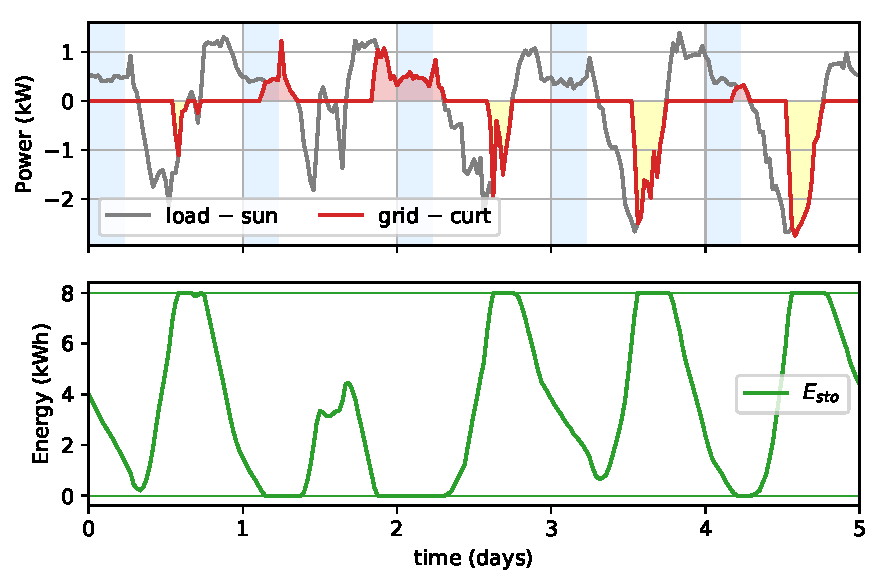
\includegraphics[width=1\columnwidth]{figures/matlab_rule-based.pdf}
    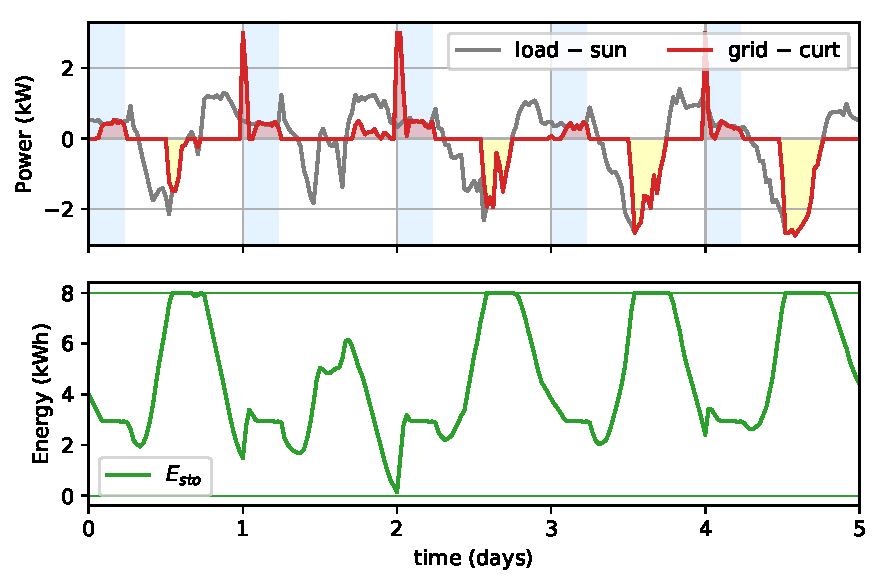
\includegraphics[width=1\columnwidth]{figures/matlab_mpc.pdf}
    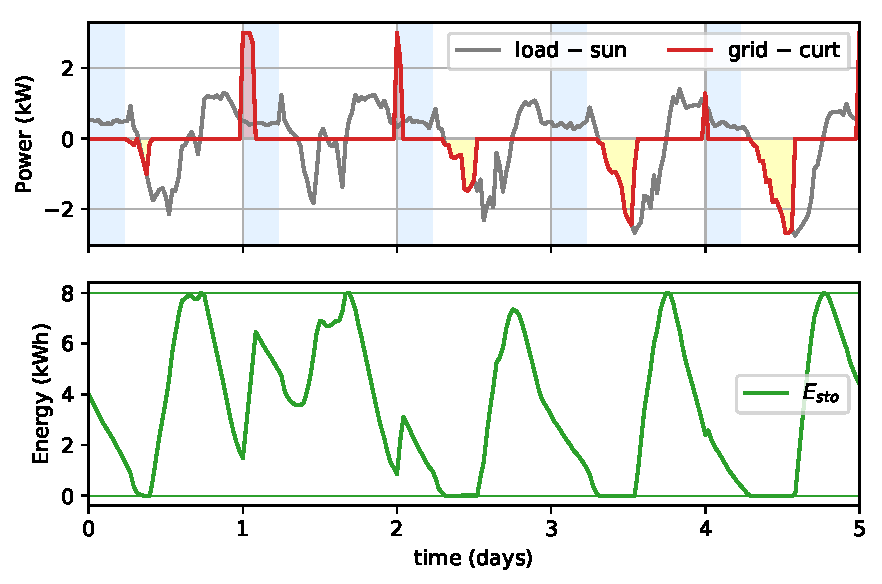
\includegraphics[width=1\columnwidth]{figures/julia_anticipative.pdf}
  \end{center}

  \caption{Tracé temporel des 5 premiers jours du test pour trois méthodes
  de gestion d'énergie de la maison solaire.
  Donnée d'entrée $P_{nl}$ en gris, décisions $P_{gc}$ en rouge (§\ref{sss:auxi_var})
  et énergie stockée $E_{sto}$ en vert.
  L'appel au réseau ($P_{gc}>0$) est rempli en rouge clair,
  alors que l'écrêtage ($P_{gc}<0$) est rempli en jaune clair.
  Les périodes bleu clair marquent les heures creuses.
  De haut en bas (du moins performant au plus performant):
  règle heuristique simple (§\ref{ss:heuris}),
  commande prédictive (MPC) avec prévision non anticipative (§\ref{ss:mpc}),
  optimisation déterministe anticipative (§\ref{ss:anticip}).
  Pour l'optimisation anticipative, la performance est artificiellement bonne,
  car la décision d'un instant dépend de données futures.
  }
  \label{fig:temporel}
\end{figure}

\subsection{Optimisation déterministe anticipative}
\label{ss:anticip}

Cette méthode consiste en une optimisation globale de la trajectoire des signaux
sur tout l'horizon du problème (30 jours pour notre test).
L'optimisation utilise la valeur observée des d'entrées incertaines,
ce qui implique que la décision sur les premiers instants dépend
de données futures.
La contrainte de non-anticipativité des décisions n'est donc pas respectée 
et la performance est donc surévaluée (c.-à-d. facture sous-évaluée).
Comme en pratique les valeurs futures des entrées incertaines ne sont pas connues,
cette méthode n'est pas implémentable in situ.

L'optimisation anticipative est utilisée dans plusieurs études scientifiques,
en particulier de dimensionnement (ex. : \cite{Rigo-Mariani:2017:ToSG}),
car elle offre une performance plus attrayante qu'une gestion empirique.
Cependant, nous pensons que cette approche est risquée, car il n'y a aucune maitrise
du niveau de sous-évaluation du coût par rapport à une gestion réelle.

Le résultat quantitatif de l'optimisation est présenté dans le tableau \ref{tab:perf_stats}
à la ligne ``optim. anticip.''.
Nous en déduisons que le minimum absolu de la facture énergétique 
(connaissant parfaitement le futur) est de 0,354\,€/j,
et cette valeur est nettement plus basse qu'avec une gestion heuristique (0,563\,€/j).

Sur le bas de la figure \ref{fig:temporel}, on peut analyser qualitativement
cette gestion d'énergie. En particulier, on observe que la recharge de la batterie
par appel au réseau se fait presque exclusivement la nuit.
Par ailleurs, la quantité d'énergie appelée dépend nettement de la production solaire
\emph{de la journée suivante} (grosse recharge nocturne si faible production future,
pas de recharge nocturne si forte production future).
L'effet d'anticipation joue donc bien un rôle important.

\subsubsection{Variante : minimisation de la consommation réseau}
Accessoirement, nous avons implémenté une variante du problème
qui optimise la consommation d'énergie réseau 
(équivalent à la minimisation de la facture si le prix était fixe).
Cette variante (ligne ``optim. éner.'' du tableau \ref{tab:perf_stats})
permet de prouver que la consommation d'énergie de 3.38\,kWh,
atteinte également par la gestion heuristique (non anticipative)
et par l'optimisation de la facture est un \emph{plancher absolu}.
Cela montre deux choses.
Premièrement, la connaissance du futur n'apporte aucun gain énergétique,
seulement un gain financier.
Deuxièmement, la minimisation de la facture se fait uniquement
par déplacements de blocs d'énergie pour mieux exploiter les
périodes de prix bas.

\subsubsection{Complexité de la résolution numérique}
\label{sss:opt_complex}

Un autre aspect important de cette optimisation est la complexité
de sa résolution numérique. Elle dépend de la \emph{convexité}
\cite{Boyd:2004:CvxOptim} du problème d'optimisation.
Pour la maison solaire, vu le modèle présenté partie \ref{ss:model},
la fonction coût est linéaire en la variable de décision $P_{grid}$,
de même que les contraintes (en particulier l'évolution de l'état d'énergie,
car on a négligé les pertes).
Le problème d'optimisation est donc du type ``programme linéaire''
(sous-classe la plus classique parmi les problèmes d'optimisation convexe)
qui se résout très efficacement malgré sa taille
($30 \times 48 = 1440$ pas de temps, avec plusieurs variables de décision).
Nous l'avons implémenté en Julia avec le package JuMP\cite{Dunning:2017:JuMP}
(outil de modélisation comparable à AMPL ou GAMS, mais implémenté en Julia
et open source).

Nous présentons à présent une variante notable de l'optimisation déterministe : la commande prédictive.
Elle a le grand avantage d'être implémentable, car les données incertaines futures y sont remplacées
par des prévisions.

\newpage

\subsection{Commande prédictive (MPC)}
\label{ss:mpc}

La commande prédictive (MPC, pour Model Predictive Control en anglais)
est une méthode très utilisée académiquement et dans l'industrie
pour la gestion d'énergie et la commande des systèmes en général\footnote{
  En toute rigueur, il faut distinguer le
  ``tracking MPC'' où l'optimisation d'une fonction coût, souvent quadratique,
  n'est qu'une façon indirecte pour suivre une trajectoire prédéfinie,
  et le ``Economical MPC'' où la minimisation du coût, pas forcément quadratique,
  et sans trajectoire fixée a priori, est l'objectif premier.
  Pour la gestion d'énergie, c'est de ce E-MPC qu'il s'agit.}.
Cette méthode se base sur une optimisation en ligne qui, \emph{à chaque pas de temps},
résout le problème d'optimisation pour en déduire une trajectoire optimale à suivre.
Pour le MPC, comme pour la programmation dynamique, le coût à minimiser est supposé
être une somme sur période longue, voire infinie,
ce qui correspond bien à la facture d'énergie \eqref{eq:C_grid} de la maison solaire.
Pour rendre le calcul d'optimisation plus rapide,
cette somme est tronquée à un nombre de pas restreint,
appelé ``horizon de prédiction'', noté $H$.
À l'instant $k$, la fonction coût à minimiser s'écrit:
%
\begin{equation} \label{eq:mpc_cost}
  J(k) = \sum_{i=k}^{k+H} c_{grid}(i)P_{grid}(i)
\end{equation} 

Cette minimisation génère une \emph{trajectoire optimale}
de toutes les variables de décision ($P_{sto}$, $P_{grid}$...)
sur la période $k$ à $k+H$.
Cependant, seule le premier instant de la trajectoire ($P_{sto}(k)$, $P_{grid}(k)$...)
est appliqué au système, car à l'instant de décision suivant,
la trajectoire est réoptimisée sur la période $k+1$ à $k+H$.
C'est une optimisation sur un \emph{horizon glissant}.
Cela permet d'utiliser les informations les plus à jour à chaque pas de temps.

Mis à part l'horizon raccourci, le problème d'optimisation
est identique à celui de l'optimisation déterministe de la partie précédente.
Comme le problème est linéaire (cf. §\ref{sss:opt_complex}) il se résout très efficacement
et la convergence est garantie, ce qui est important pour une mise en oeuvre
(à noter tout de même que le système de commande doit embarquer un solveur linéaire).

Par contre l'optimisation est effectuée à chaque pas de temps,
ce qui rallonge le temps de simulation sur la période de test.
Lorsque l'on souhaite répéter les simulations de nombreuses fois en phase
de dimensionnement, cela peut être prohibitif,
d'où l'usage de la gestion heuristique partie \ref{ss:dimens}.

Un dernier point positif important est à souligner pour le MPC :
il est très flexible.
Ainsi, l'ajout d'une formule de prix plus complexe (ex. : heures de pointe)
ne changerait en rien sa structure.

\subsubsection{Prévision des entrées incertaines}

Dans la partie précédente (§\ref{ss:anticip}), nous avons souligné
qu'une optimisation qui utilise des données futures n'est pas utilisable
en pratique. Cependant, la fonction coût du MPC \eqref{eq:mpc_cost} dépend des
mêmes données futures, quoique sur un horizon plus court.
Toute commande prédictive nécessite donc une méthode de \emph{prévision des entrées incertaines}.

Pour la maison solaire, nous avons pour l'instant testé deux prévisions :
\begin{itemize}
 \item prévision anticipatrice, c'est-à-dire la connaissance parfaite du futur sur l'horizon $H$
 \item prévision réaliste simple égale à la moyenne à chaque heure du jour
 ($hod = 0, 0.5, ..., 23.5$) sur les données passées
 (les 30 jours d'apprentissage correspondant au mois précédent le test, cf. §\ref{ss:sol_data}).
\end{itemize}

La prévision anticipatrice est inapplicable en pratique, mais elle permet
de comparer le MPC à l'optimisation déterministe (§\ref{ss:anticip} qui travaille,
elle, sur toute la durée du problème.
Cela permet donc d'étudier l'effet de la troncature du coût  à un horizon $H$

La prévision réaliste est présentée figure \ref{fig:pred}.
On peut constater que la prévision est meilleure pour la consommation
que pour la production solaire. En effet, la production solaire présente
une plus forte variabilité. Par exemple à midi solaire, la moyenne est à 2\,kW
pour une production réelle allant de presque 0 à plus de 3\,kW.

On constate accessoirement une certaine \emph{persistance} des signaux,
c'est-à-dire que l'erreur de prévision est autocorrélée.
Cette persistance à l'échelle de quelques heures pourrait permettre
d'améliorer la prévision.

\begin{figure}
        \begin{center}
                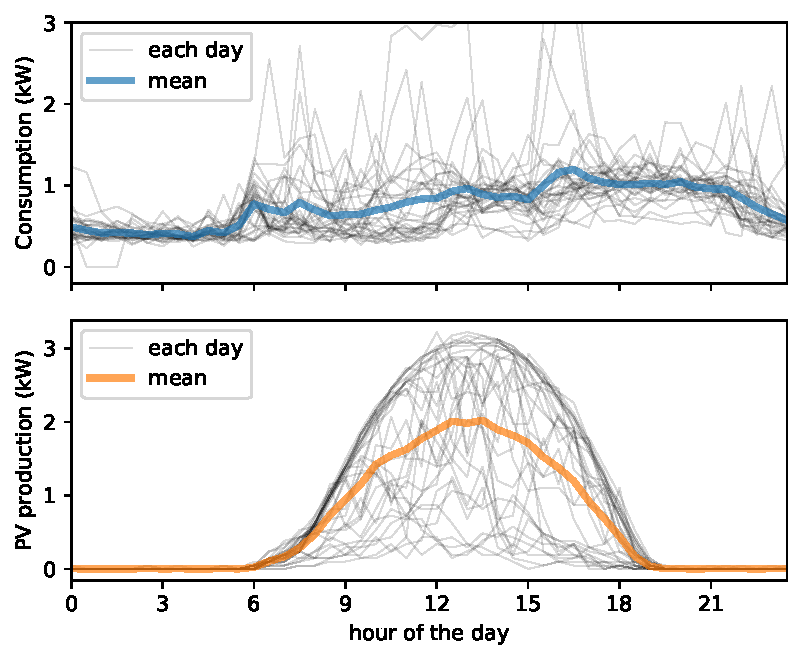
\includegraphics[width=1\columnwidth]{figures/daily_traj_M-1-2011-11-28_PV4kWp.pdf}
        \end{center}

        \caption{Prévision de la consommation $P_{load}^*$ et du productible $P_{sun}$
        (pour une puissance des panneaux $P_{PVp}$ = 4\,kW\sub{c})
        par calcul de la moyenne à chaque heure du jour, par pas d'une demi-heure,
        sur les 30 jours d'apprentissage.
        La superposition des trajectoires de chaque jour permet de constater
        que l'erreur de prévision est potentiellement grande, surtout pour la production.
        }
        \label{fig:pred}
\end{figure}

\subsubsection{Effet de la prévision sur la performance}

Le résultat quantitatif de la gestion MPC est présenté dans le tableau \ref{tab:perf_stats}
aux lignes ``MPC...''. L'horizon $H$ a été choisi égal à 24\,h ($H \times \Delta_t = 24$\,h).
Nous constatons qu'avec la prévision anticipatrice, le coût de la facture énergétique
atteint 0,354\,€/j, comme l'optimisation sur les 30 jours.
Avec un horizon de 24\,h, l'effet de la troncature du coût est donc nul.

Par contre, nous observons également qu'avec la prévision réaliste (ligne ``MPC 24 h''),
la dégradation de la performance est notable : +1\,kWh/j sur la consommation d'énergie
associé à une augmentation identique de l'écrêtage du productible solaire :
l'insertion de la production solaire est dégradée.
Quant à la facture, elle atteint 0,543\,€/j, ce qui est plus faible,
même si très proche, de celle de la gestion heuristique (0,563\,€/j).
À ce stade nous ne savons pas si cette différence est significative ou non
(i.e. robuste vis-à-vis d'un changement des données d'entrées).

Le tracé du milieu de la figure \ref{fig:temporel} permet d'analyser qualitativement
la gestion d'énergie MPC avec prévision réaliste.
On constate que, face à une journée qui est toujours prévue identique, 
la gestion d'énergie utilise systématiquement le début de nuit (heure creuse) pour amener la batterie
à un état d'énergie autour de 3\,kWh.
On imagine que cela doit permettre de tenir sans appel au réseau sur toute la journée prévue.
En pratique, si la journée est nuageuse (jour 2), un appel au réseau supplémentaire
est nécessaire en fin de journée (au tarif heure pleine).
Inversement, si la journée qui suit est très ensoleillée (jour 4),
la charge nocturne aurait pu être évitée, mais il est trop tard
et c'est l'écrêtage qui s'active.

\subsubsection{Réglage de l'horizon de prédiction}
La longueur de l'horizon prédiction $H$ (nombre de pas entier,
mais que nous exprimons en heures, comme $H \times \Delta_t$)
est un paramètre essentiel de toute commande prédictive.
Pour le régler, nous l'avons fait varier entre 0 et 48\,h,
et les résultats sont présentés sur la figure \ref{fig:mpc_horiz}.
Vu l'effet important de la prévision, les deux types précédents
ont été utilisés (anticipative et réaliste).

Dans le cas de la prévision anticipative, la consommation électrique
reste largement constante pour toutes les valeurs de l'horizon $H$,
tandis que le coût décroît jusqu'à sa valeur minimale (0,354\,€/j),
valeur atteinte dès $H.\Delta_t = 19$\,h.
Ce seuil s'interprète comme la durée minimale de l'horizon glissant qui permet de couvrir
à tout instant une partie de la tranche d'heures creuses de deux journées consécutives.
Ainsi, la recharge nocturne peut être parfaitement ajustée à la production/consommation
attendue pour la journée suivante.

Par contre lorsqu'on utilise la prévision réaliste, l'augmentation
de l'horizon a un effet inattendu : la performance se dégrade,
dès qu'on dépasse 3\,h. 
Le tracé de l'énergie consommée sur le réseau montre une augmentation forte de la consommation moyenne
lorsque l'horizon passe de 20 à 24\,h.
Nous supposons donc que le MPC fait une réserve nocturne pour pallier un manque
de soleil attendu.
Cette augmentation de la consommation se voit aussi sur le coût de l'énergie,
même s'il n'augmente que lentement, autour de 0.55\,€/j.
Cette augmentation le fait diverger du coût obtenu avec une prévision anticipatrice parfaite.

Ainsi, le MPC qui se base sur une optimisation déterministe
(les données prévues sont supposées se réaliser) se fait piéger
par l'erreur de prévision.
Les pistes d'améliorations sont donc de deux ordres:
amélioration de la prévision d'une part
(mais difficile, car on pressent que le facteur important est la balance énergétique
de toute la journée suivant chaque nuit)
et formulation du problème d'optimisation qui prend en compte les inévitables
erreurs de prévisions (MPC stochastique, robuste...).

\begin{figure}
        \begin{center}
                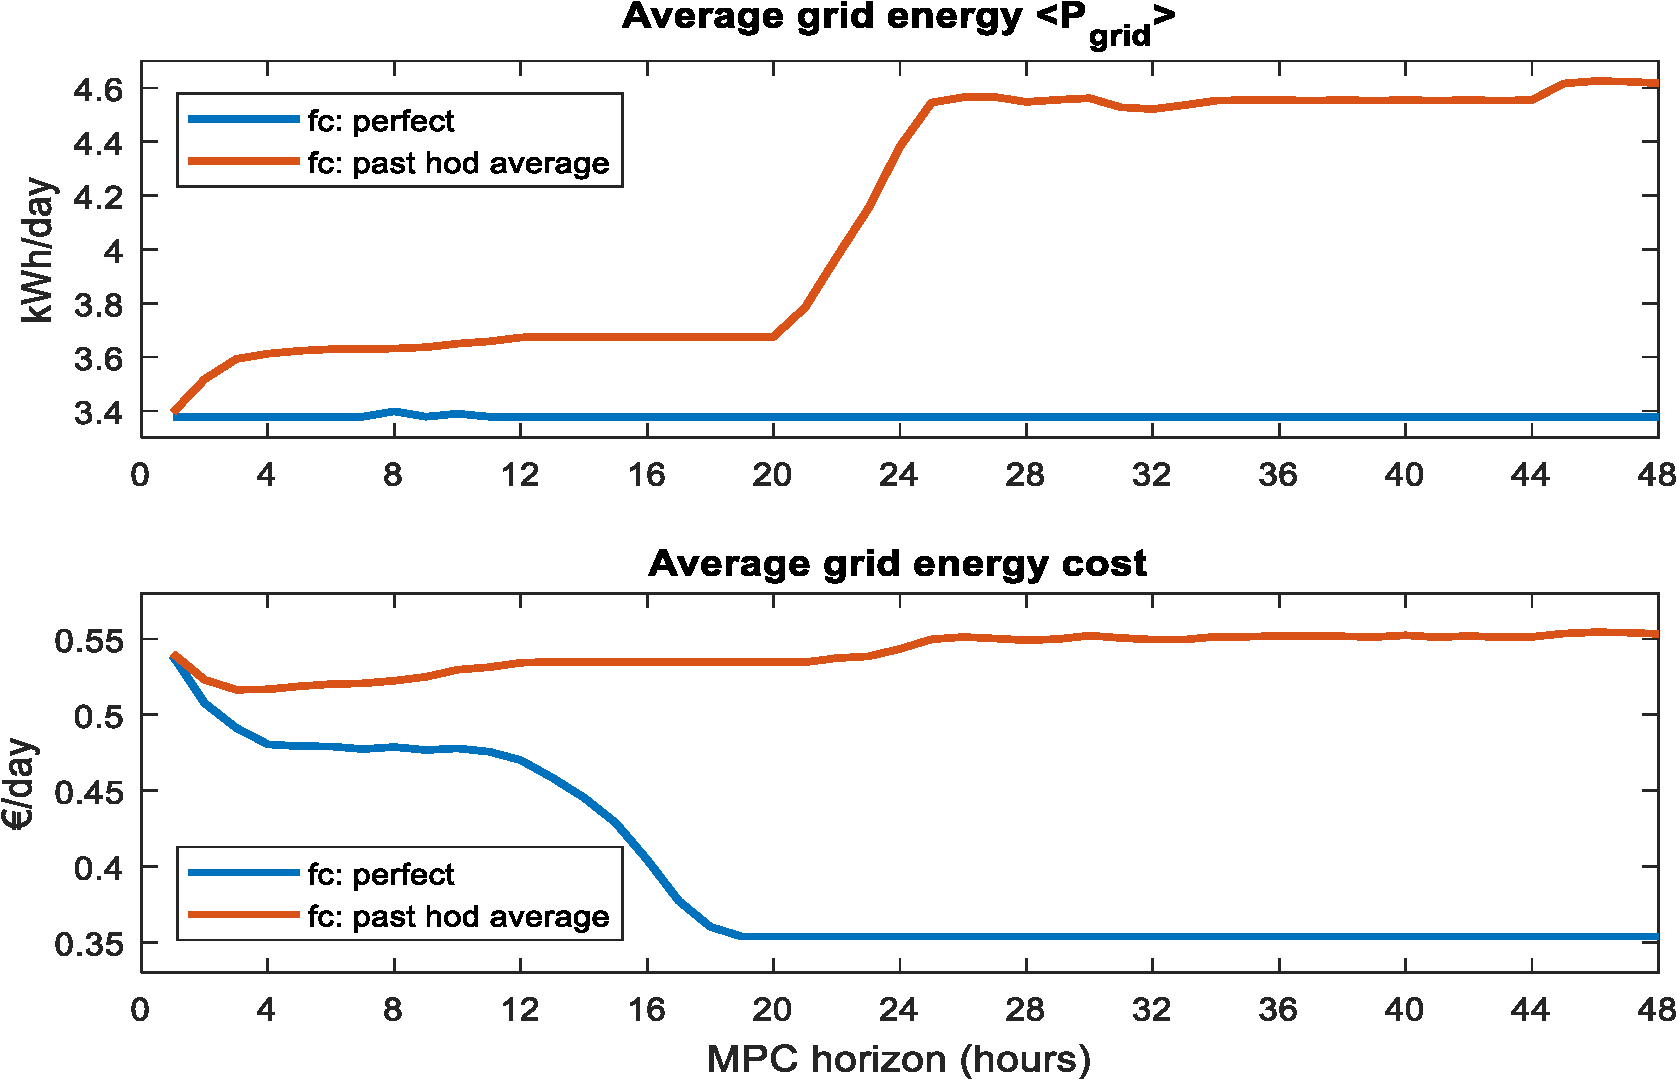
\includegraphics[width=1\columnwidth]{figures/MPC_horizon_effect.pdf}
        \end{center}

        \caption{Effet de l'horizon du contrôle MPC sur la performance
        (consommation d'énergie réseau en haut, coût de cette énergie en bas).
        Courbes bleues: MPC alimenté par une prévision parfaite (anticipative) du futur.
        Courbes rouges: MPC alimenté par une prévision réaliste, égale à la moyenne passée à chaque heure du jour. 
        }
        \label{fig:mpc_horiz}
\end{figure}

% \subsection{Commande prédictive non-linéaire}
% 
% Optimica JModelica.org \cite{Akesson:2010:CCE}

\section{Conclusions}

Nous avons conçu un banc de test open source pour la gestion d'énergie d'une maison solaire.
Il facilite l'accès et permet la comparaison d'une palette de méthodes,
sur un exemple simple mais réaliste (e.g. données de production solaire et de consommation réelles).

Les premières stratégies de gestion que nous avons implémentées et comparées
font ressortir quelques idées attendues
(ex. : les méthodes heuristiques simples donnent de bons résultats sur les problèmes simples).
D'autres résultats sont nettement moins courants, comme l'effet délétère
de l'allongement de l'horizon de prédiction sur la performance d'une commande prédictive.
Autrement dit, une prédiction longue, lorsqu'elle est partiellement fausse, est pire qu'une courte.

Plus généralement, nous avons fait ressortir le grand écart qui existe
entre la performance de stratégies anticipatives (qui supposent connaitre le futur des données incertaines)
et la performance des méthodes qui n'utilisent que des données connues.
Seules ces dernières sont implémentables sur un système réel!

\subsection{Perspectives}
Parmi les perspectives de ces travaux, il y a bien sûr l'ajout de nouvelles méthodes
de gestions d'énergie.
Nous visons en particulier les méthodes qui prennent en compte intrinsèquement
le caractère incertain des données solaire et de consommation:
programmation dynamique stochastique, MPC stochastique...

À plus longue échéance, nous souhaitons aller au-delà
des tests de gestion d'énergie à dimensionnement fixé.
Nous souhaitons étudier les méthodes de dimensionnement optimal
qui prennent en compte l'optimisation de la loi de gestion
(comme nous l'avions fait sur un cas nettement plus simple \cite{Haessig:2014:SGE}).

% structure de décision dans un contexte multi-agent (pas abordé ici
% car focus sur optimisation d'un système individuel) : centralisé, distribué,
% mécanisme de prix, multi-agent...

\bibliographystyle{IEEEtran}
\bibliography{00_References}

\end{document}